\chapter{绪论}
\label{chapter:intro}

\section{研究背景}
\label{section:background}

生物信息学是研究生物信息的采集、处理、存储、传播和解释等各方面的学科。
生物信息学可以帮助人类从海量的生物数据中挖掘内部的生理过程规律,从而指导进一步的生物学研究。在规模化实验大力发展和海量数据爆发的如今,如何有效的利用生物数据变得越来越中了。
生物信息学分为三个主要的发展阶段,前基因组时代主要建立了各种生物数据库和序列比较算法、基因组时代进行了大规模的基因测序以及目前所处的后基因组时代。
后基因组时代研究重心以生物数据分析为主,并且挖掘的层次逐渐深入。已经从对基因组直接的结构的研究逐渐转向对基因功能的研究,其中的主要侧重点包括基因组学、转录组学以及蛋白质组学等\cite{helms_principles_2019}。

蛋白质是生物细胞和组织的重要组成部分,是生命体的物质基础,也是遗传信息的直接表达手段,涉及生物体载体、免疫、激素等方方面面。蛋白质分子深度参与了组织的构成与修复、生理功能的调节和能量的供给。
蛋白质组学\cite{schubert_quantitative_2017}是在蛋白质表达层面研究生理生化功能为主的一门学科,目的是揭示蛋白质的基本生命活动规律,其中研究主要关注蛋白质结构、蛋白质丰度、蛋白质修饰以及蛋白质相互作用。

蛋自质在细胞活动中发挥着巨大的作用。但是在多数情况下单个蛋自质无法独立的执行生物功能,只有构成蛋白质复合物,才能有效的参与到细胞活动中\cite{gavin_functional_2002}。因此蛋白质复合物的结构、功能及形成方式的研究就显得尤为重要。图\ref{fig:swr1_complex}是具有染色质重塑功能的酵母SWR1复合物。
\begin{figure}[htbp]
  \centering
  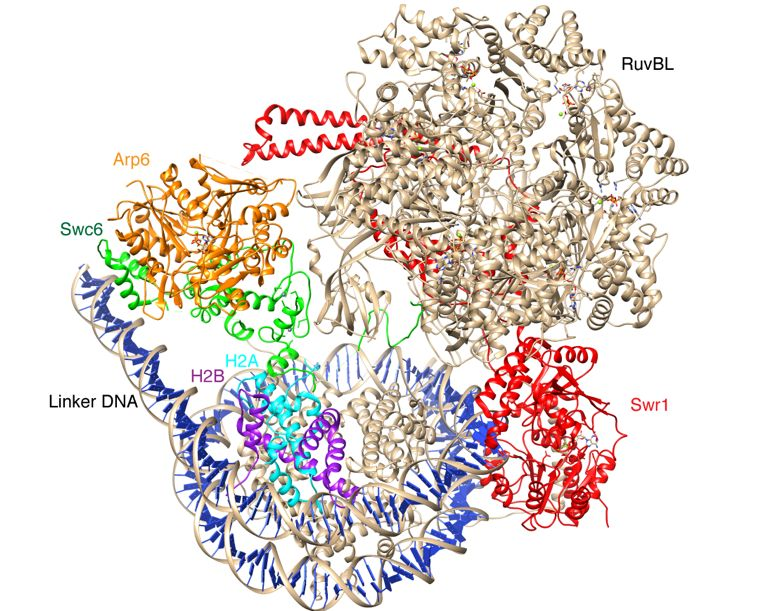
\includegraphics{SWR1_complex}
  \caption{酵母菌SWR1复合物}
  \label{fig:swr1_complex}
\end{figure}
生物实验中检测蛋白质复合物主要通过串联亲和纯化与质谱分析\cite{g_generic_1999}、酵母双杂交\cite{li_identification_1993}两种技术对蛋白质复合物进行分离和鉴定。串联亲和纯化与质谱分析通过靶蛋白标定以及自然条件下亲和纯化获取可能的蛋白质复合物,再使用质谱分析进行鉴定。酵母双杂交技术利用转录调控因子中的组件特征研究蛋白质之间的相互作用关系。虽然基于实验测定的方法具有生物学上的可解释性,但是生物实验往往条件困难、实验步骤多且成本昂贵,无法满足快速增长的研究需求。

蛋白质与生理环境存在广泛的相互作用,蛋白质复杂功能的实现同蛋白质之间、DNA与蛋白质、RNA与蛋白质的相互作用密切相关,蛋白质复合物正是一组强相关的蛋白质组合共同作用的结果。随着生物信息学的发展以及高通量技术的发展,蛋白质相互作用关系(Protein-ProteinInteraction,$PPI$,后简称为互作关系)得到了大量的补充,促成了大规模互作网络的构建\cite{butland_interaction_2005},即蛋白质相互作用网络(Protein-ProteinInteractionNetwork,$PIN$)。图\ref{fig:ppi}为酵母菌蛋白质相互作用网络。
\begin{figure}[htbp]
  \centering
  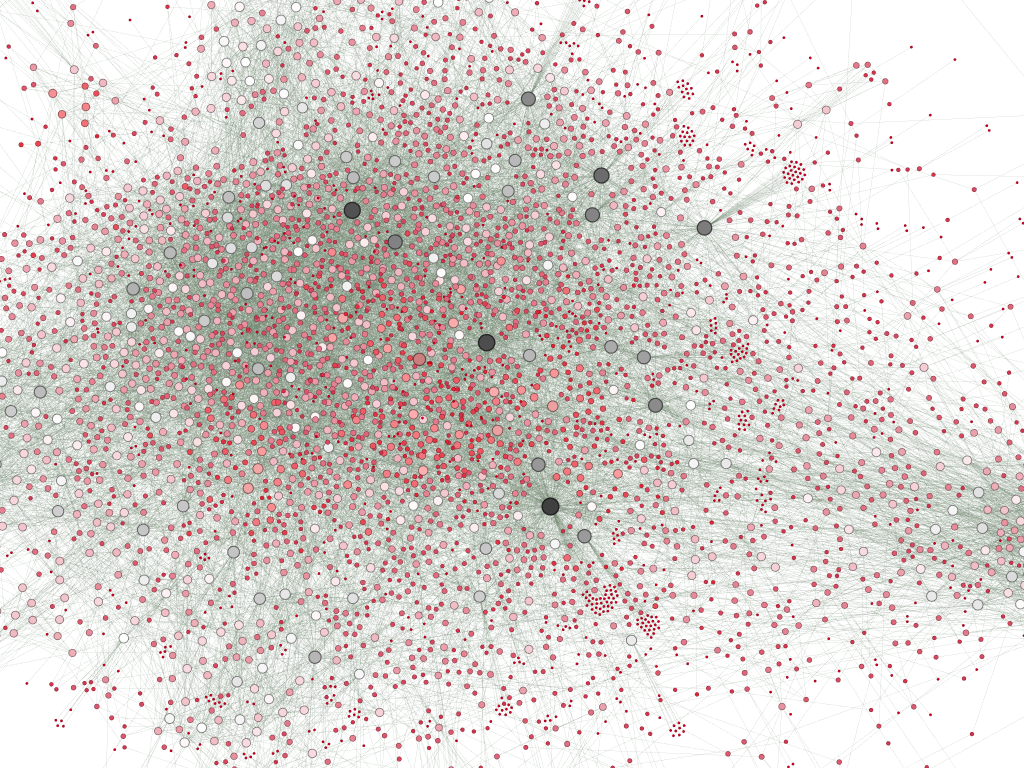
\includegraphics[width=10cm]{ppi-dip-color}
  \caption{酵母菌蛋白质相互作用网络}
  \label{fig:ppi}
\end{figure}
已知的蛋白质复合物可以视作互作网络里面的一系列子网络,因此利用图论和计算模型学习子网络的分布模式,即可在互作网络中发掘潜在的蛋白质复合物\cite{legrain_proteinprotein_2001}。利用图论的方法,蛋白质互作网络可以转换为无向图~$G=(V,E)$。其中$V$为图中结点的集合,表示所有的蛋白质,$E$为图中邻边的集合,表示所有的蛋白质互作关系。$PIN$转换为图结构之后,图论上的计算模型和深度学习方法就可以迁移到蛋白质复合物的研究中。2002年,Tong\cite{tong_combined_2002}等人提出了密集子图的假说,蛋白质复合物在$PIN$是密集链接的子图,而与其他的蛋白质连接相对稀疏。在$PIN$中预测蛋白质复合物的问题就转换为了密集子图的挖掘问题,逐渐发展出了利用$PIN$和计算方法识别蛋白质复合物的理论。

\section{国内外研究现状}
\label{section:research}

现有的基于计算方法的蛋白质复合物预测方法主要分为五类:基于网络结构的图聚类方法、融合生物信息的图聚类方法、核心附属扩展方法、动态网络方法以及监督学习方法。以下分别对这五类方法的研究现状做简单的介绍。

\subsection{基于网络结构的图聚类方法}
\label{subsection:TopologyMethod}

现有大多数复合物预测方法为基于网络结构的图聚类方法,基本思路是在无权无向图中挖掘密集子图。这类方法较为简单明确,取得了一定的成果。

MCODE算法\cite{bader_automated_2003}是最早提出基于网络结构构造密集子图的复合物预测算法。首先算法会计算所有结点的局部邻居密度,其中密度超过平均值的结点成为种子,视作初始子图。满足相应阈值条件的邻居结点不断扩充子图,直到阈值条件饱和,最终子图视为预测的复合物,算法最终会过滤掉结点数少的复合物。
Clique算法\cite{spirin_protein_2003}通过穷举法、超顺磁性聚类和蒙特卡洛模拟三种方法搜索完全图来检测蛋白质复合物。
RNSC算法\cite{king_protein_2004}以随机聚簇最为初始聚簇,按照代价函数逐渐削减聚簇,最终形成蛋白质复合物。
Pereira‐Leal\cite{pereiraleal_detection_2004}提出将马尔科夫聚类算法应用于蛋白质复合物检测,通过转移矩阵的自乘来扩展连通区域,通过幂运算进行膨胀操作只保留生成概率高的区域。膨胀和扩展操作交替运行,收敛之后获得蛋白质复合物。
LCMA算法\cite{li_interaction_2005}从$PIN$中较小的完全图开始,通过不断合并重合率高的完全图来检测蛋白质复合物。CFinder算法\cite{adamcsek_cfinder_2006}进一步定义了搜索与合并的策略,算法首先寻找网络中的k阶完全图,如果两个子图之间有k-1个公共结点,则定义为两个k阶完全图相邻,将两个子图合并。算法通过不断合并k阶完全图预测蛋白质复合物。
SCAN算法\cite{mete_structural_2008}认为一对蛋白质的公共邻居超过阈值时,这对蛋白质可被视为结构可达,可以作为种子蛋白质继续扩展其余结构可达蛋白质。
ClusterONE算法\cite{nepusz_detecting_2012}充分利用了蛋白质复合物内部连接密集,外部连接稀疏的假设,并且明确定义了子图紧密性。其主要思路是首先按照结点度排序获取种子结点,种子结点向外扩展操过程中可以添加或删除结点,以达到局部子图最佳紧密性。
Zheng等人\cite{zheng_protein_2020}进一步改进了图紧密性定义,提出根据子图中3阶完全图个数来定义局部子图连紧密性。

有部分研究将$PIN$中的结点做预分类以达到更优的结果。
CPridict算法\cite{xu_function_2014}首先计算蛋白质之间的功能相似性,然后$PIN$以功能相似性做谱聚类,将蛋白质分为多个分组,各个分组独立进行复合物预测。CPridict2.0算法\cite{xu_effective_2017}进一步基于FunCat功能目录对蛋白质进行分组。
CODEC算法\cite{geva_identification_2011}基于质谱实验将蛋白质分类为诱饵蛋白和靶标蛋白,从靶标蛋白及其邻居结点开始,通过增减结点获得最大子图得分。

\subsection{网络预处理的图聚类方法}
\label{subsection:appendBiology}
蛋白质复合物的预测是一个复杂的生物学问题,而由于实验手段的限制,互作数据存在着高假阴性和高假阳性的缺陷\cite{von_mering_comparative_2002}。研究者开始尝试挖掘网络拓扑特征,对网络结构进行修复和连边加权处理,提高$PIN$的可信度以获取更精确的聚类结果。
DPClus算法\cite{altaf-ul-amin_development_2006}最早对$PIN$做加权处理,根据一对结点公共邻居数量给这对结点之间的边加权,结点的权重所有邻边的权重之和。权重较大的结点作为种子结点,通过紧密型结点的连接预测蛋白质复合物。
PCP算法\cite{chua_using_2008}利用使用FS-weight计算邻边的可靠度,并移除网络中可靠度较低的边,之后利用完全图发现合并算法检测复合物。
CMC算法\cite{liu_complex_2009}采用了一种迭代式的边加权方法,不断的以结点的加权公共邻居数更新邻边权重,完全图评价分数也和子图的权重有关。
Bootstrap算法\cite{friedel_bootstrapping_2009}基于boostrap采样法预测复合物,在网络中做有放回重复采样,多次采样确定蛋白质相互作用权重,再进行多次执行马尔可夫聚类算法,形成蛋白质聚簇。最终以蛋白质在聚簇网络中的贡献性重构$PIN$权重。

除了基于拓扑结构的加权方法,还可以利用生物信息对相互作用加权。已有研究表明\cite{komurov_revealing_2007},形成功能团的蛋白质通常具有相同的基因表达。部分研究借助基因表达数据更改权重,重新定义密集子图的评价函数以达到更优的聚类效果。
MATISSE算法\cite{ulitsky_identification_2007}使用基因表达数据的相关性衡量蛋白质的互作强度,并以此定义$PIN$的权重,再将聚类算法运用到加权网络预测蛋白质复合物。
GFA算法\cite{jianxing_feng_max-flow-based_2011}基于最密子图算法获取互作网络中的最密子图,将子图的密度定义为子图内基因表达量之和,在聚类结果中选取密度较大的子图为复合物。

蛋白质复合物中,蛋白质的功能表达往往趋向于相近或者相同,因此功能表达数据也有助于蛋白质相互作用加权。Lubovac等人\cite{lubovac_combining_2006}在基因本体信息\cite{ashburner_gene_2000}(GENE Ontology,简称GO)形成的有向无环图上,使用SWEMODE算法计算两个蛋白质的功能相似性。在$PIN$中结点权重通过聚合邻边权重以及邻居数计算,后续借鉴MCODE在结点和邻边均加权的网络中预测蛋白质复合物。WCOACH算法\cite{kouhsar_wcoach_2016}同样使用蛋白质功能表达数据加权,在加权网络上运用改进的COACH算法\cite{leung_predicting_2009}。

有研究表明,蛋白质结构域互作信息也会对蛋白质复合物的形成产生影响\cite{kim_relating_2006},多对蛋白质无法作用于互作界面的重复区域。Jung等人\cite{jung_protein_2008}利用这个特性,剔除了MCODE和LCMA生成的结果中具有结构域冲突的复合物,提高了结果的准确性。DACO算法\cite{will_identifying_2014}将蛋白质相互作用和结构域相互作用数据结合起来,使用图聚类算法预测蛋白质复合物时,进行结构域的紧密优化,预测出来的复合物确保存在结构域互作的可能性。


\subsection{核心附属扩展方法}
\label{subsection:CoreAppend}

SCAN算法\cite{mete_structural_2008}已经提出了基于种子蛋白质扩展的复合物预测方法。然而种子蛋白质仅仅时拓扑结构上的聚类核心,并不具有明显的生物学意义。研究人员\cite{gavin_proteome_2006}通过酵母菌中复合物的结构发现,部分蛋白质存在于多种复合物中,且这些蛋白质之间存在大量的相互作用关系,组成了复合物的功能单元,此类蛋白质被称为核心蛋白质。在一个复合物中其余蛋白质附着于核心蛋白质,被称为附属蛋白质。如图\ref{fig:core_append}所示,其中深色椭圆形底框部分为复合物中的核心模块。

CORE算法\cite{leung_predicting_2009}是基于蛋白质复合物核心附属形成机理提出的算法,通过计算两个蛋白质公共邻居之间互作情况发现核心蛋白质,通过核心蛋白质周围相互作用关系添加附属蛋白质。COACH算法\cite{leung_predicting_2009}根据蛋白质及邻居在$PIN$网络中的重要程度确定核心蛋白质,其中蛋白质结点权重越大,其成为核心蛋白质的可能性越高。

\begin{figure}[htbp]
  \centering
  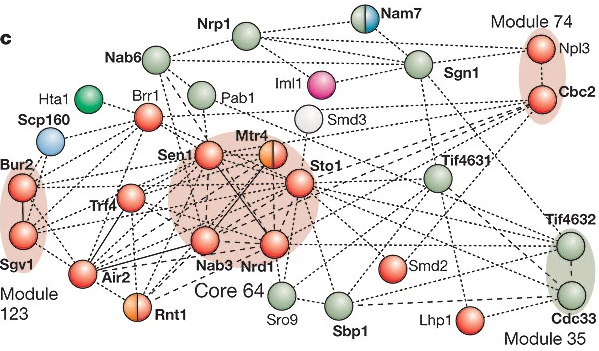
\includegraphics{core_append}
  \caption{核心附属结构示例——Core64部分为核心结构}
  \label{fig:core_append}
\end{figure}

\subsection{监督学习方法}
\label{subsection:Supervision}
这里多突出一个后处理
包括监督下的方法
刘晓霞
\subsection{动态网络方法}
\label{subsection:Dynamic}

由于蛋白质会随着生理生化周期不断变化,因此蛋白质相互作用也具有动态特性,部分研究\cite{li_dynamic_2017}将基因表达时序数据和蛋白质相互作用结合,构建动态蛋白质相互作用网络$Dynamic-PIN$。
Tang等人\cite{tang_comparison_2011}设定阈值,将蛋白质基因表达数据超过阈值的蛋白质视为活跃蛋白质,以活跃蛋白质构建动态网络。Ou-Yang等人\cite{ou-yang_detecting_2014}使用基因表达数据区分瞬态和稳态蛋白质。

\subsection{方法总结}
\label{subsection:researchSummary}

表\ref{}给出了现有方法的类别、思想以及相关特点。



\section{研究动机和思路}
\label{section:motivation}

国内外学者对复合物的识别已经提出了诸多方法,总体趋势也是趋向于融合生物数据和网络数据并达到更精确的预测,但是目前现有的方法还存在以下的不足。
\begin{itemize}

  \item 无法充分利用已有的先验知识。上述的研究方法主要是基于无监督方法,在复合物的研究问题上,无监督方法具有训练简单、结构明确的优点。但是随着实验技术更新、生物数据量增加以及图数据挖掘算法的井喷发展,无监督学习方法无法利用已有的先验知识,其预测准确率无法得到进一步提升。有监督学习方法可以通过学习已有复合物的分布特征,挖掘出特定$PIN$网络中蛋白质复合物的分布规律。目前已有的监督方法如Shi提出的方法\cite{shi_protein_2011}仅仅学习复合物的拓扑特征的映射函数,且映射函数只作用于复合物扩展过程中单个结点的取舍判断,算法尚存在大量的改进空间。

  \item 复合物准确度较低。部分模型方法如RNSC算法\cite{king_protein_2004}、Clique算法\cite{spirin_protein_2003}等等具有很强的随机性,此类方法为了达到较高的复合物召回率,往往倾向于产生过量的候选复合物,导致结果的准确率的降低。预测的复合物中存在大量错误的样本,对后续的生物研究有一定的影响。如何在维持复合物预测召回率的情况下,提高预测的准确度是一个值得研究的问题。

  \item 生物信息在$PIN$中融合度低。在\ref{subsection:appendBiology}中提到了融合生物信息的诸多方法,然而这些方法只停留在利用生物信息更改$PIN$邻边权重的层面,不同的生物信息如GO注释、基因表达信息、蛋白质保守性等数据被统一编码到了相互作用的边权重中,这个编码转换过程会丢失原有丰富的生物数据。编码过程仅仅作为$PIN$数据的预处理,生物数据无法动态地参与到复合物预测模型的框架设计中。同时,目前也没有方法将生物信息编码到蛋白质结点中,如何有效的利用结点编码增强复合物的预测质量也是一个亟待解决的问题。
\end{itemize}

针对以上的问题,本文提出了一种基于监督学习和融合特征的复合物筛选模型。

算法的核心思想是利用已有的生物数据,包括$PIN$、生物注释信息、已知复合物等等,通过监督学习的方式构建一个鲁棒性的复合物分类模型。模型能够较为准确的辨别某一个复合物是否为真实复合物。在此模型训练成功的前提下,将一般性的复合物预测算法,比如DPClus算法\cite{altaf-ul-amin_development_2006}、MCODE算法\cite{bader_automated_2003}等产生的复合物交由分类模型做进一步筛选,相当于filter过程,剔除其中得分较低的样本,保留得分高的样本作为预测的最终结果。由于无效样本的剔除,理论上经过filter的处理,最终预测结果的多项评价指标可以提升。

这种二阶段筛选方法在目标检测领域已经得到了广泛的运用。
RNSC算法\cite{king_protein_2004}最早提出过基于设定得分函数筛选预测复合物的思想,,Clique算法\cite{spirin_protein_2003}过多样本,Pereira‐Leal\cite{pereiraleal_detection_2004}融合了总体拓扑结构,论文\cite{yu_predicting_2014}filter the candidate complexes

刘晓霞。。。

\section{研究工作及成果}
\label{section:workandresult}

基于以上的研究思路,本文进行了以下的具体研究,并取得了相应的研究成果。

\section{论文组织}
\label{section:organization}